\documentclass[12pt,twocolumn]{article}
\usepackage[margin=0.7in]{geometry}
\usepackage{graphicx}
\usepackage{cite}
\linespread{1.5}
                                        
%%%%%%%%%%%%%%%%%%%%%%%%%%%%%%%%%%%%%%%%%%%%%%%%%%%%%%%%%%%%%%%%%%%%%%%%%%%%%%%%%%%%%%%%%%%%%%%%%%%%%%%%%%%%%%%%%%%%%%%%%%%%%%%%%%%%%%%%%%%%%%%%%%%%%%%%%%%%%%%%%%%%%%%%%%%%%%%%%%%%%%%%%%%%%%%%%%%%%%%%
                                        
\begin{document}
\title{Muons}
\author{Joseph Hartsell and M. Lane}
\date{\today}

\maketitle


\begin{abstract}
Using a Teach Spin Scintillator, mean muon lifetime was measured by histogram decay half-time measurements in this experiment. The muon proper lifetime was determined to be 2.198 $\mu$s. The rate of
measured muon flux was compared with known values to verify relativistic time-dilation
effects and we examined briefly the Fermi Constant.
\end{abstract}

\section{Introduction}
 Muons are a negatively charged lepton similiar to the electron except with 200 times the mass. It is most frequently found in cosmic radiation.  The first time the muon decay was measure was in 1941 when  F. Rasetti showed that muon’s have a finite ”lifetime” now known to be 2.19 μs \cite{COSBUL}. Today thanks to the particle data group we know the value to actually be 2.196981 ± 0.000002 μs \cite{COSBUL}. The muon, along with its positively charged counterpart the antimuon are the make up the second lepton group.
Muons are often the by product of decay of negative pions that decay them selves from decay of free protons in the atomosphere. Figure below is has sketch of these primary decays of cosmic ray radiation, which naturally occurs in Earth’s upper at- mosphere due to primary cosmic rays interac- tions with air molecules. Cosmic rays include protons, neutrons, pions, kaons, and other particles from the air is not understood well [2]; suffices to know that pions are released which spon- taneously decay into a muon and neutrino via the processes below [2] and as shown on the figure:
In turn muons naturally decay is :

Muons are a negatively charged elementary particle similar to a heavy electron. In 1941,
F. Rasetti demonstrated that muon's have a finite "lifetime" now known to be 2.197$\mu$s
. Where lifetime is related to the half-life decay rate.
The muon, along with its positively charged counterpart the anti-muon, is
classified as a lepton.

Muons are often created from the decay of pions, which naturally occurs in Earth's upper
atmosphere due to primary cosmic rays interactions with air molecules. The complete process
in which primary cosmic rays liberate protons, neutrons, pions, kaons, and other particles
from the air is not understood well \cite{MUON}; however, it suffices to know that pions are released
which spontaneously decay into a muon and neutrino via the processes below \cite{MUON}.

\begin{equation}
	\label{eq:PionDecay}
	\begin{array}{c}
	\pi^{+}\rightarrow\mu^{+}\nu_{\mu} \\
	\pi^{-}\rightarrow\mu^{-}\bar{\nu}_{\mu}
\end{array}
\end{equation}

The muons produced travel at speeds near 99.9\% the speed of light \cite{PDG}. Takeing their production
altitude is 15km above sealevel\cite{PDG} and assuming they travel normal to Earth's surface we expect
the travel time to reach earth is then: $15km/c = 50\mu s$. Much larger than their mean lifetime.

The fact that any significant number of muons have been detected on Earth's surface indicates that they
cannot have a mean lifetime of $2.2\mu s$ and travel time of $50\mu s$. We take this as evidence for time
dilation.

Instead muons experience a time dilation given by $t'=t_{0}/\gamma$, with $\gamma=\left(1-\beta^{2}\right)^{-1}$.
With the speed given above, we then expect muons to experience a travel time 500times less than previously
predicted. A much more reasonable estimate. 

To truly calculate the travel time in the muon's reference frame, we must also account for the
speed loss as the muon travels through a medium. The energy loss for a muon as it travels
through a constant density fluid as given by T.E. Coan and J. Ye\cite{MUON} is:

\begin{equation}
	\label{eq:decaytime}
	\Delta E = 2 MeV/g/cm^{2} \cdot H \cdot \rho
\end{equation}

Where $\rho$ is the fluid density and $H$ is the height traveled through. We then note that
$dE=\rho C_{0} dh$, and from Einstein's relation we have $E=\gamma mc^{2}, dE=mc^{2}d\gamma$
which gives:

\begin{equation}
	dh = \frac{mc^{2}}{\rho C_{0}} d\gamma
\end{equation}

Noting that the travel time in the particle's rest frame is given by $dt'=dh / \left( c\beta\gamma \right)$
then gives:

\begin{equation}
	t' = \frac{mc}{\rho C_{0}} \int_{\gamma_{1}}^{\gamma_{2}} \frac{ d\gamma }{ \beta\gamma } = \frac{mc}{\rho C_{0}} \int_{\gamma_{1}}^{\gamma_{2}} \frac{ d\gamma }{ \sqrt{ \gamma^{2}-1 } }
\end{equation}


\begin{equation}
	t' = \frac{mc}{\rho C_{0}} \left.\log\left(\sqrt{\gamma^{2}-1}+\gamma\right)\right|_{\gamma_{1}}^{\gamma_{2}}
\end{equation}

This is useful for a number of simple calculations. Firstly, muons reach the Earth's surface with a kinetic enery near 4GeV
 corresponding to $\gamma_{1}=38$. Using $\Delta E$ from Eq. \ref{eq:decaytime}, we find the energy and gamma factor in the
 upper atmosphere to be $\gamma_{2}=54.$ Using these values as the integral bounds gives a reasonable $t'=1.18\mu s$ in agreement with
 the first order calculation.

 Given also that muons decay at a constant rate in any medium, we have $dN=\lambda dt$. This gives the familiar
 equation:
 \begin{equation}
	 \label{eq:probability}
	 N=N_{0}exp(-\lambda t)
 \end{equation}
 
 Where $\lambda$ is used to define the mean lifetime as $\lambda=1/\tau$.  This can 
 now be used to determine a height difference necessary for an experiment. Suppose we wished to measure and
 compare muon counts at two different elevations. For a noticable difference between the two locations, we will say
 the time difference for the muon between the two locations should be $t'\approx 0.10\cdot\tau$ which gives $1-e^{-0.1}\approx10\%$
difference in muon counts between the two locations.

By using $t'=0.1\tau$ we find $\Delta\gamma\approx15=\Delta E / mc^2$. Which is nearly the same change experienced from
the height of the atmosphere to sea-level. To truly perform a elevation varying experiment, very sensitive equipment should
be used and a difference in muon counts less than 1\% must be able to be accurately measured.

In this experiment, we will use Eq. \ref{eq:probability} to measure the mean proper lifetime of muons. First note that
the probability distribution is exponential, a memoryless probability distribution. This means the muons we may detect
in the laboratory will decay under the same distribution despite having already traveled through the atmosphere. By
fitting an exponential to measured decay times, we may measure the proper mean lifetime.

\section{Method}

In order to detect muon decays, we will utilizie a plastic scintillator. When a charged particle enters the scintillator
it will begin to slow, emitting light as it looses energy. A photodetector then begins a timer when a flash indicates
a particle has entered. If a muon enters with sufficiently low kinetic energy, it will stop inside the scintillator and
decay. When it decays, it emits photons which tells the photodetector to stop the timer. In this way, the time needed
for a muon to decay is measured. If no secondary flash is detected within a brief period, the particle is assumed
to have passed through without decaying, or is not a muon and not recorded as an event.

\begin{figure}[h!]
	\centering
	\label{fig:scin}
	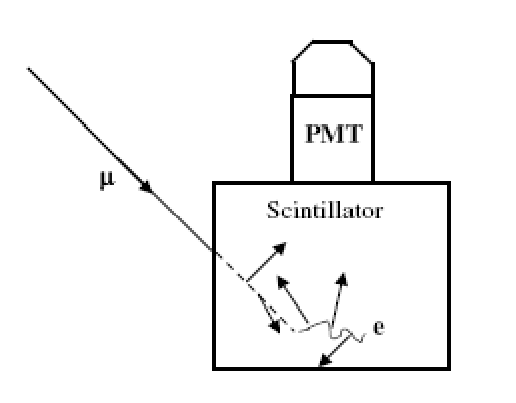
\includegraphics[width=3in]{images/scintillatorevents}
	\caption{Photon emission used in determining the lifetime of a muon}
\end{figure}

The scintillator was connected to a computer which recorded the time of each event, and the time (in nanoseconds) between
the initial flash and decay flash of a given event. The events were set to record beginning at 3:00pm on June 5th, 2012
and were collected every Tuesday and Thursday until data collection was halted at 6:00pm June 19th, 2012.

\section{Analysis}

The data collected only consisted of the time between entering and decaying in nanoseconds. This was converted into a 
probability distribution by creating a histogram from the data. The initial histogram is shown below.

\begin{figure}[h!]
	\centering
	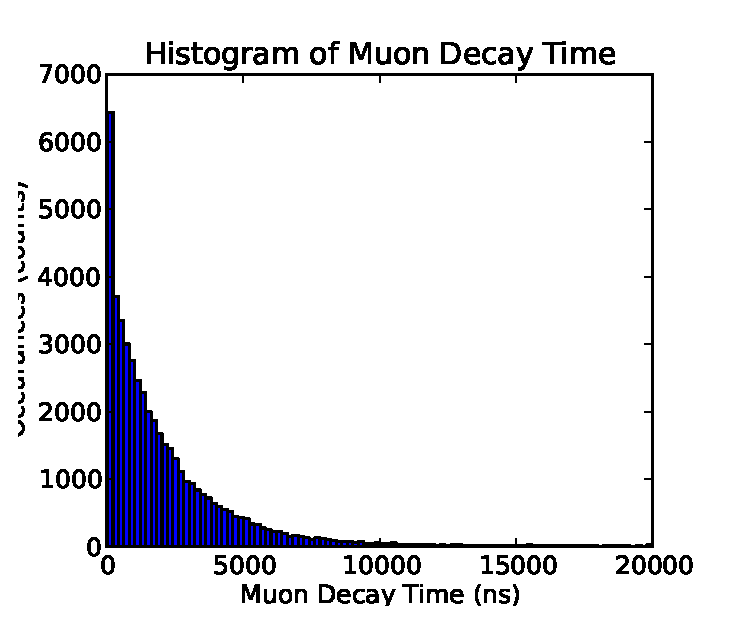
\includegraphics[width=3in]{images/Histogram}
	\caption{Raw Histogram}
	\label{fig:Histogram}
\end{figure}

With some foresight that the proper lifetime is near $2\mu s$, we mas safely assume that counts above $10\mu s$ are
noise and interference and should not be included in the analysis. Therefore, to calculate proper lifetime, we take
the logarithm of Eq. \ref{eq:probability} to obtain:

 \begin{equation}
	 \label{eq:probability}
	 \log(N)=\frac{-t}{\tau} + \log(N_{0})
 \end{equation}

 The data is then plotted on semi-log axes and a line fit to the data. The slope of the line gives the decay rate while
 the intercept is related to the counts recieved. As will be discussed in the error analysis section, the initially 
 calculated lifetime is used to estimate the background noise. The background noise is then subtracted out and the fit
 calculation redone. Using this method we found the slope of the fit line to be -0.4550 indicating $\tau=2.1978$ in
 agreement with known values.

\begin{figure}[h!]
	\centering
	\label{fig:fit1}
	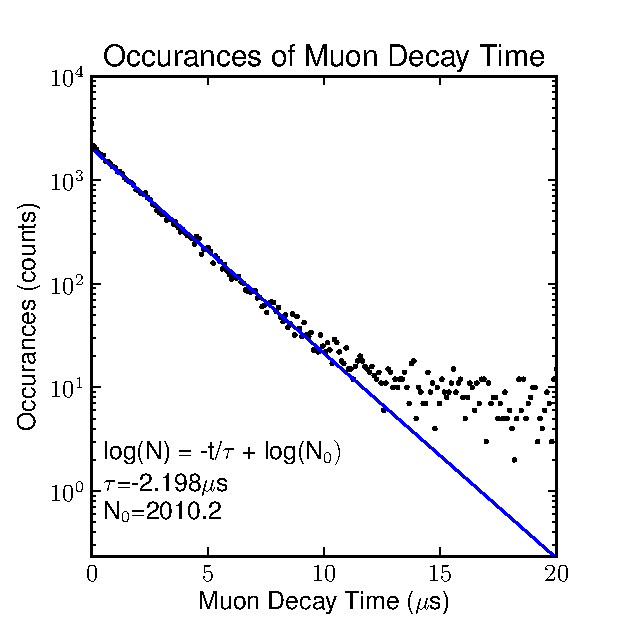
\includegraphics[width=3in]{images/fit1}
	\caption{Histogram with fit equation}
\end{figure}

\section{Error Analysis}

This experiment is very prone to false positives because a muon decay is only recognized by sufficiently quick
flashes within the scintillator. It is very likely that many recorded events are not a decay, but two particles
passing through in the same time period. It is assumed however, that any "coincidental events" will not occur
preferentially to a specific time range. They shift the entire distribution vertically upward and not affect the shape of
the graph.

To compensate for this, we may take an initial estimate of the lifetime and perform a fit as shown in Fig. \ref{fig:fit1}.
Notice the fit holds for small times, but above $5\tau$ noise becomes significant. Therefore we take the background noise to be
a constant number of counts for each bin of the histogram and calculate it by averaging the deviation from measured and fit
for values of $t>5\tau$.

To obtain a confidence estimate for our measurement of $\tau$, we look to the coefficient of determination of the linear
regression. The fit performed has: $r^{2}=0.992$ indicating the linear fit is well formed in the low-t region. We will say
that a reasonable fit requires $r^{2}>0.98$, and found that a 5\% variation in $\tau$ caused $r^{2}$ to drop below the 
threshold value. Therefore, we assert that $\tau=2.2\pm5\%$.

\nocite{*}
\bibliography{references}
\bibliographystyle{plain}
\end{document}
